\documentclass{article}
\usepackage{tikz}
\begin{document}
\begin{titlepage}
    \centering
    \vspace*{2cm}
    {\Huge\bfseries Assignment 7\par}
    \vspace{2cm}
    {\Large Amarnath Patel\par}
    \vfill
    {\large 7/29/2024 \par}
\end{titlepage}

\section*{Question 1}

Consider a graph \( G \) consisting of vertices \( V = \{v_1, v_2, v_3, v_4\} \) and edges \( E = \{e_1 = (v_1, v_2), e_2 = (v_2, v_3), e_3 = (v_3, v_1), e_4 = (v_3, v_4)\} \).

\subsection*{(a) Is \( G \) directed or undirected? Justify your answer.}
The graph \( G \) is undirected because the edges are given as unordered pairs of vertices. In directed graphs, edges are ordered pairs indicating direction.

\subsection*{(b) Draw \( G \) and label each vertex and edge accordingly.}
\begin{center}
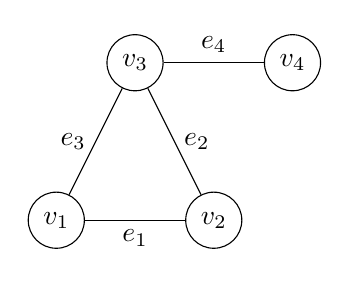
\begin{tikzpicture}
    \node[circle, draw] (v1) at (0, 0) {$v_1$};
    \node[circle, draw] (v2) at (2, 0) {$v_2$};
    \node[circle, draw] (v3) at (1, 2) {$v_3$};
    \node[circle, draw] (v4) at (3, 2) {$v_4$};
    
    \draw (v1) -- (v2) node[midway, below] {$e_1$};
    \draw (v2) -- (v3) node[midway, right] {$e_2$};
    \draw (v3) -- (v1) node[midway, left] {$e_3$};
    \draw (v3) -- (v4) node[midway, above] {$e_4$};
\end{tikzpicture}
\end{center}

\subsection*{(c) Determine the degree of each vertex in \( G \).}
\begin{itemize}
    \item Degree of \( v_1 \): 2 (connected to \( v_2 \) and \( v_3 \))
    \item Degree of \( v_2 \): 2 (connected to \( v_1 \) and \( v_3 \))
    \item Degree of \( v_3 \): 3 (connected to \( v_1 \), \( v_2 \), and \( v_4 \))
    \item Degree of \( v_4 \): 1 (connected to \( v_3 \))
\end{itemize}

\subsection*{(d) Is \( G \) connected? Why or why not?}
The graph \( G \) is connected because there is a path between any pair of vertices. For example:
\begin{itemize}
    \item \( v_1 \) to \( v_4 \): \( v_1 \to v_3 \to v_4 \)
    \item \( v_2 \) to \( v_4 \): \( v_2 \to v_3 \to v_4 \)
\end{itemize}

\section*{Question 2}
\subsection*{(a) Define a multigraph and explain how it differs from a simple graph.}
A multigraph is a graph that allows multiple edges between two vertices. In other words, it is a graph that can have parallel edges. This means that there can be more than one edge connecting the same pair of vertices. In contrast, a simple graph only allows one edge between any two vertices.

\subsection*{(b) Example of a multigraph with a loop and multiple edges between two vertices.}
Consider a multigraph \( G' \) consisting of vertices \( V' = \{v'_1, v'_2, v'_3\} \) and edges \( E' = \{e'_1 = (v'_1, v'_2), e'_2 = (v'_2, v'_3), e'_3 = (v'_2, v'_3), e'_4 = (v'_3, v'_3)\} \).

\subsection*{(c) Real-world scenario represented by the multigraph.}
This multigraph could represent a transportation network where the vertices represent different locations and the edges represent different routes between the locations. For example, \( v'_1 \) and \( v'_2 \) could be two cities connected by multiple highways, while \( v'_3 \) could be a city with a loop road system. The multiple edges between \( v'_2 \) and \( v'_3 \) could represent different routes or lanes within the city. The loop edge \( e'_4 \) could represent a circular road within the city.

\section*{Question 3}

Given the following list of edges in a directed graph: \{(A, B), (B, C), (C, D), (D, A), (B, D), (C, A)\},

\subsection*{(a) Draw the directed graph.}
\begin{center}
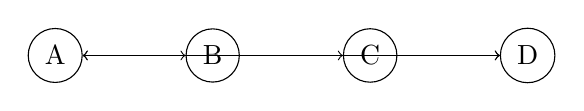
\begin{tikzpicture}
    \node[circle, draw] (A) at (0, 0) {A};
    \node[circle, draw] (B) at (2, 0) {B};
    \node[circle, draw] (C) at (4, 0) {C};
    \node[circle, draw] (D) at (6, 0) {D};
    
    \draw[->] (A) -- (B);
    \draw[->] (B) -- (C);
    \draw[->] (C) -- (D);
    \draw[->] (D) -- (A);
    \draw[->] (B) -- (D);
    \draw[->] (C) -- (A);
\end{tikzpicture}
\end{center}

\subsection*{(b) Identify any circuits within the graph. If any, classify them as simple or not.}
There is a circuit in the graph: A -> B -> C -> D -> A. This circuit is simple because it does not repeat any vertices or edges.

\subsection*{(c) Does this graph have an Euler path or circuit? Justify your answer.}
This graph does not have an Euler path or circuit. In order for a directed graph to have an Euler path, it must have at most one vertex with outdegree - indegree = 1 and at most one vertex with indegree - outdegree = 1. In this graph, both vertex A and vertex D have outdegree - indegree = 1, and both vertex B and vertex C have indegree - outdegree = 1. Therefore, there is no Euler path or circuit in this graph.

\section*{Question 4}
\subsection*{(a) How many edges does the tournament graph have?}
In a tournament graph with n vertices, the number of edges can be calculated using the formula: \( \frac{{n \cdot (n-1)}}{2} \).
For a tournament graph with 5 vertices, the number of edges is \( \frac{{5 \cdot (5-1)}}{2} = 10 \).

\subsection*{(b) Is it possible for every vertex in a tournament graph to have the same degree? Explain.}
No, it is not possible for every vertex in a tournament graph to have the same degree. In a tournament graph, each vertex has a different outdegree and indegree. The outdegree of a vertex represents the number of edges leaving the vertex, while the indegree represents the number of edges entering the vertex. Since there is exactly one directed edge between each pair of distinct vertices in a tournament graph, the degrees of the vertices will be different.

\subsection*{(c) Can a tournament graph be a simple graph? Justify your answer.}
No, a tournament graph cannot be a simple graph. A simple graph is an undirected graph that does not have any parallel edges or self-loops. In a tournament graph, there is exactly one directed edge between each pair of distinct vertices, which means there are parallel edges. Additionally, since the edges in a tournament graph are directed, there are no self-loops. Therefore, a tournament graph cannot be a simple graph.

\section*{Question 5}
\subsection*{(a) Draw both G1 and G2.}
\begin{center}
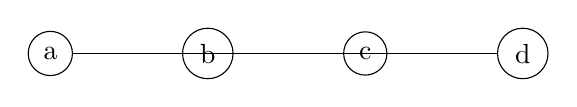
\begin{tikzpicture}
    \node[circle, draw] (a) at (0, 0) {a};
    \node[circle, draw] (b) at (2, 0) {b};
    \node[circle, draw] (c) at (4, 0) {c};
    \node[circle, draw] (d) at (6, 0) {d};
    
    \draw (a) -- (b);
    \draw (b) -- (c);
    \draw (c) -- (d);
    \draw (d) -- (a);
    \draw (a) -- (c);
\end{tikzpicture}
\end{center}

\begin{center}
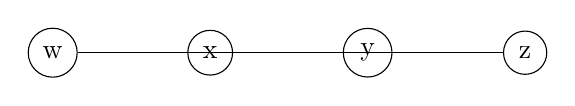
\begin{tikzpicture}
    \node[circle, draw] (w) at (0, 0) {w};
    \node[circle, draw] (x) at (2, 0) {x};
    \node[circle, draw] (y) at (4, 0) {y};
    \node[circle, draw] (z) at (6, 0) {z};
    
    \draw (w) -- (x);
    \draw (x) -- (y);
    \draw (y) -- (z);
    \draw (z) -- (w);
    \draw (w) -- (y);
\end{tikzpicture}
\end{center}

\subsection*{(b) Assess whether G1 and G2 are isomorphic.}
To determine if G1 and G2 are isomorphic, we need to define a function f : V(G1) → V(G2) to map vertices from G1 to G2, and a function h : E(G1) → E(G2) to map edges from G1 to G2.

Let's define the functions:
f(a) = w
f(b) = x
f(c) = y
f(d) = z

h((a, b)) = (w, x)
h((b, c)) = (x, y)
h((c, d)) = (y, z)
h((d, a)) = (z, w)
h((a, c)) = (w, y)

Now, let's verify if f and h form a one-to-one correspondence:
For every edge e = (u, v) in E(G1), there is an edge h(e) = (f(u), f(v)) in E(G2).

For example, let's take the edge (a, b) in G1. f(a) = w and f(b) = x. h((a, b)) = (w, x), which is an edge in G2.

Similarly, we can verify that for every edge in G1, there is a corresponding edge in G2 based on the vertex mapping f.

Therefore, G1 and G2 are isomorphic.

\end{document}